\documentclass{article}

\usepackage{fancyhdr}
\usepackage{extramarks}
\usepackage{amsmath}
\usepackage{amsthm}
\usepackage{amsfonts}
\usepackage{tikz}
\usepackage[plain]{algorithm}
\usepackage{algpseudocode}
\usepackage{enumitem} 

\usetikzlibrary{automata,positioning}

%
% Basic Document Settings
%

\topmargin=-0.45in
\evensidemargin=0in
\oddsidemargin=0in
\textwidth=6.5in
\textheight=9.0in
\headsep=0.25in

\linespread{1.1}

\pagestyle{fancy}
\lhead{\hmwkAuthorName}
\chead{\hmwkClass\: \hmwkTitle}
\rhead{\firstxmark}
\lfoot{\lastxmark}
\cfoot{\thepage}

\renewcommand\headrulewidth{0.4pt}
\renewcommand\footrulewidth{0.4pt}

\setlength\parindent{0pt}

%
% Create Problem Sections
%

\newcommand{\enterProblemHeader}[1]{
    \nobreak\extramarks{}{Exercício \arabic{#1} continua na próxima página\ldots}\nobreak{}
    \nobreak\extramarks{Exercício \arabic{#1} (continuação)}{Exercício \arabic{#1} continua na próxima página\ldots}\nobreak{}
}

\newcommand{\exitProblemHeader}[1]{
    \nobreak\extramarks{Exercício \arabic{#1} (continuação)}{Exercício \arabic{#1} continua na próxima página\ldots}\nobreak{}
    \stepcounter{#1}
    \nobreak\extramarks{Exercício \arabic{#1}}{}\nobreak{}
}

\setcounter{secnumdepth}{0}
\newcounter{partCounter}
\newcounter{homeworkProblemCounter}
\setcounter{homeworkProblemCounter}{1}
\nobreak\extramarks{Exercício \arabic{homeworkProblemCounter}}{}\nobreak{}

%
% Homework Problem Environment
%
% This environment takes an optional argument. When given, it will adjust the
% problem counter. This is useful for when the problems given for your
% assignment aren't sequential. See the last 3 problems of this template for an
% example.
%
\newenvironment{homeworkProblem}[1][-1]{
    \ifnum#1>0
        \setcounter{homeworkProblemCounter}{#1}
    \fi
    \section{Exercício \arabic{homeworkProblemCounter}}
    \setcounter{partCounter}{1}
    \enterProblemHeader{homeworkProblemCounter}
}{
    \exitProblemHeader{homeworkProblemCounter}
}

%
% Homework Details
%   - Title
%   - Due date
%   - Class
%   - Section/Time
%   - Instructor
%   - Author
%

\newcommand{\hmwkTitle}{Lista de Exercícios\ \#1}
\newcommand{\hmwkDueDate}{March 22, 2024}
\newcommand{\hmwkClass}{Álgebra Linear}
\newcommand{\hmwkClassTime}{} 
\newcommand{\hmwkClassInstructor}{}% {Professor Isaac Newton}
\newcommand{\hmwkAuthorName}{\textbf{Tiago da Silva}}

%
% Title Page
%

\title{
    \textmd{\textbf{\hmwkClass:\ \hmwkTitle}}\\
    \normalsize\vspace{0.1in}\small{Due\ on\ \hmwkDueDate}\\
    \large{\textit{\hmwkClassInstructor\ \hmwkClassTime}}
}

\author{\hmwkAuthorName}
\date{}

\renewcommand{\part}[1]{\textbf{\large Part \Alph{partCounter}}\stepcounter{partCounter}\\}

%
% Various Helper Commands
%

% Useful for algorithms
\newcommand{\alg}[1]{\textsc{\bfseries \footnotesize #1}}

% For derivatives
\newcommand{\deriv}[1]{\frac{\mathrm{d}}{\mathrm{d}x} (#1)}

% For partial derivatives
\newcommand{\pderiv}[2]{\frac{\partial}{\partial #1} (#2)}

% Integral dx
\newcommand{\dx}{\mathrm{d}x}

% Alias for the Solution section header
\newcommand{\solution}{\textbf{\large Solution}}

% Probability commands: Expectation, Variance, Covariance, Bias
\newcommand{\E}{\mathrm{E}}
\newcommand{\Var}{\mathrm{Var}}
\newcommand{\Cov}{\mathrm{Cov}}
\newcommand{\Bias}{\mathrm{Bias}}

\begin{document}

% \maketitle

% \pagebreak
\begin{homeworkProblem} \label{ex:a} 
    \begin{figure}
        \centering
        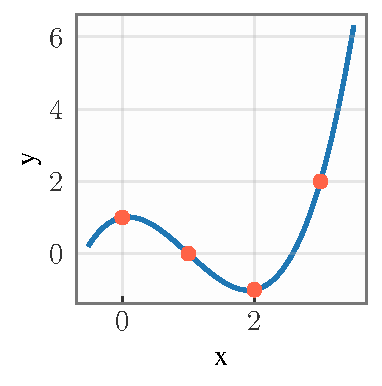
\includegraphics[width=.5\textwidth]{figures/pol.pdf}
        \caption{Figura para o Exercício 1.}
        \label{fig:a}
    \end{figure}
    O bem conhecido teorema de interpolação de polinômios de Lagrange garante a existência de um polinômio de grau $n$ cujo gráfico contém quaisquer $n + 1$ pontos dados em $\mathbb{R}^{2}$ com abscissas distintas. Para o caso apresentado, definimos 
    \begin{equation}
        p(x) = \sum_{1 \le i \le 4} x^{i - 1} a_{i - 1}  
    \end{equation}
    e notamos que o problema de encontrar $(a_{i - 1})_{1 \le i \le 4}$ tal que o gráfico de $p$ contém $\{ P_{i} \colon 1 \le i \le 4\}$ é equivalente a resolver 
    \begin{equation} \label{eq:a} 
        p(P_{i}[1]) = P_{i}[2] \text{ para } 1 \le i \le 4, % . 
    \end{equation}
    em que $P[1] = x$ e $P[2] = y$ se $P = (x, y)$. Note que \eqref{eq:a} é um sistema linear em $(a_{i - 1})_{1 \le i \le 4}$. Veja a \ref{fig:a} para o polinômio resultante da solução deste sistema. 
\end{homeworkProblem}

\pagebreak 

\begin{homeworkProblem}
    Sejam $n_{x}, n_{y}, n_{z}$ o número de aquisições em milhares quotas $x, y, z$ respectivamente. 
    \begin{enumerate}[label=(\alph*)]  
        \item As condições de Asdrúbal serão satisfeitas se 
        \begin{equation}
            \begin{cases}
                n_{x} + n_{y} + 3 n_{z} = 3.8, \\
                n_{x} + 2 n_{y} + 4 n_{z} = 5.2, \\ 
                n_{x} + 3 n_{y} + 7 n_{z} = 9. 
            \end{cases}
        \end{equation}
        A terceira equação deste sistema é igual à soma da primeira e da segunda e, em particular, ele é indeterminado; há uma infinidade de soluções. Em particular, qualquer tripla em 
        \begin{equation} \label{eq:aa} 
            \left\{ (2.4 - 2 n_{z}, 1.4 - n_{z}, n_{z}) \colon n_{z} \in \mathbb{R} \right\}   
        \end{equation}
        satisfaz o problema. Para derivar este resultado, basta resolver as duas equações iniciais do sistema; a solução garantidamente satisfaz a equação restante. 
        \item Uma solução que satisfaz é $n_{x} = 0$, $n_{y} = 0.2$ e $n_{z} = 1.2$, obtida substituindo $n_{z} = 1.2$ em \eqref{eq:aa}. 
    \end{enumerate} 
\end{homeworkProblem}

\end{document}
